\documentclass[a4paper]{iacas}

\usepackage{cite}
\usepackage{hyperref}% embedding hyperlinks [must be loaded after dropping]
\usepackage{amsmath,amsthm,amssymb,amsfonts,latexsym,mathrsfs,wasysym}
\usepackage{marvosym}
\usepackage{subcaption}
\usepackage{soul,color}
\usepackage{threeparttable}% tables with footnotes
\usepackage{dcolumn}% decimal-aligned tabular math columns
\usepackage{float}
\usepackage{graphicx}
\usepackage{accents}
\usepackage{tikz}
\usepackage{lastpage}
\usepackage{fancyhdr}
\usepackage{color}
\usepackage{cancel}
\usepackage{setspace}
\usepackage{enumitem}
\usepackage{pdfpages}
\usepackage{algorithm}
\usepackage{algorithmic}


%\doublespacing
% or:
\onehalfspacing
%\usepackage[T1]{fontenc}
%\usepackage{bigfoot} % to allow verbatim in footnote
\usepackage[framed,numbered]{matlab-prettifier}
\pagestyle{plain}
%\usepackage[hebrew,english]{babel}
\usetikzlibrary{shapes.geometric, arrows, calc}

\newcolumntype{d}{D{.}{.}{-1}}
\graphicspath{{figures/}}

% define some commands to maintain consistency
\newcommand{\pkg}[1]{\texttt{#1}}
\newcommand{\cls}[1]{\textsf{#1}}
\newcommand{\file}[1]{\texttt{#1}}
\newcommand{\sgn}[1]{\operatorname{sgn}\left(#1\right)}
\newcommand{\sat}[1]{\operatorname{sat}\left(#1\right)}
\newcommand{\rrule}[1]{\rule[#1]{0pt}{0pt}}
\newcommand{\fracds}[2]{\frac{\displaystyle #1\rrule{-0.2em}}{\displaystyle #2\rrule{1em}}}
\newcommand{\figref}[1]{Fig.~\ref{#1}}
\newcommand{\ubar}[1]{\underaccent{\bar}{#1}}
\newcommand{\norm}[1]{\lvert \lvert \vec #1 \rvert \rvert}

%diffeomorphism

\begin{document}

\begin{center}
 \large Image processing - 046200
 \end{center}
\begin{center}
\large\textbf{Homework \#4}
 \end{center}


\begin{tabular}{l}
\\
{\bf\textit{Alexander Shender 328626114}} \\
{\bf\textit{Sahar Carmel 305554453}} \\
Technion - Israel Institute of Technology
\end{tabular}


\newpage
\section{Question 1.}
\subsection{}
Since the radius is constant, the parameters space is decreased to 2 parameters: \textit{a} and \textit{b}. The dimensions are 2D:

\begin{equation*}
\{a,b\} \in R^{2}
\end{equation*}
\subsection{}
Given R=4, we are mapping all the possible circles with this radius which may have this point (which is given on the graph) on its perimeter. Meaning that any point on the circle which we drew (e.g. $a_{i}, b_{i}$) may be the center of a circle, which will include the main point given.

\begin{figure}[h!]
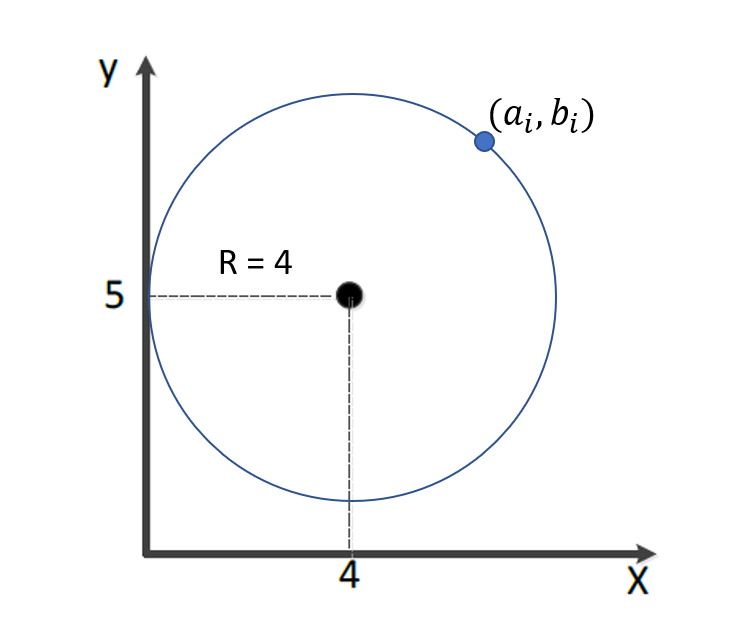
\includegraphics[scale=0.7]{imgs/q1_1.png}
\end{figure}

\subsection{}
For each of those points A, B, C - we draw a circle around with a given radius R=2. We can see that there are 3 intersections between the circles, marked as p1, p2, p3. Which means:
\begin{enumerate}
\item p1 - can be a center of a circle which includes points A and B. It got 2 votes
\item p2 - can be a center of a circle which includes points B and C. It got 2 votes
\item p3 - can be a center of a circle which includes points A, B and C. It got 3 votes
\end{enumerate}

\begin{figure}[h!]
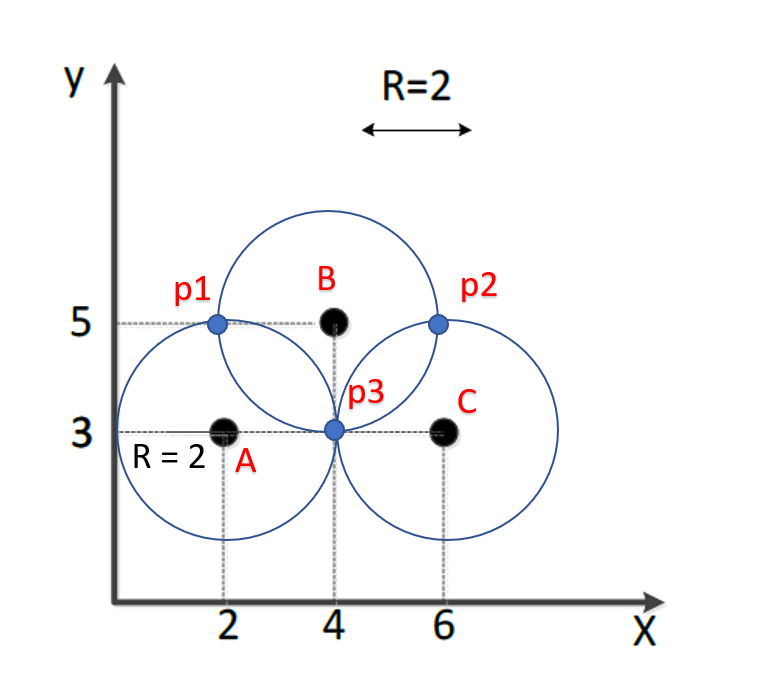
\includegraphics[scale=0.7]{imgs/q1_3.png}
\end{figure}


\subsection{}
Yes, as we have seen, point p3 can be the center of a circle which includes all 3 points. The coordinates of p3 are (4,3), and the visualization of a circle is the following:
\begin{figure}[h!]
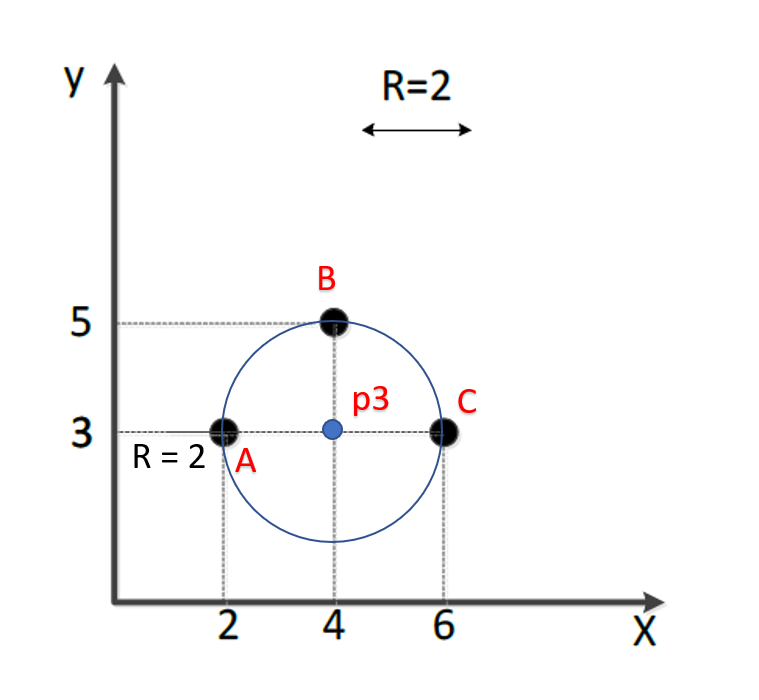
\includegraphics[scale=0.7]{imgs/q1_4.png}
\end{figure}


\subsection{}

The algorithm is divided into 2 parts . First part is the CHT transform on the image. Let us assume we have N points, and we do the transform on all of them:
\newpage
\algsetup{indent=1em}
\begin{algorithmic}[1]
\FOR{i = 1 \TO N points } 
\STATE \FOR{ $\theta$ = 0 \TO 360 deg (step = $\delta \theta$)} 
	\STATE {
\begin{equation*}
\begin{aligned}
a &= x_{i} + R\cdot cos(\theta) \\
b &= y_{i} + R\cdot sin(\theta) \\
A[a,b] &+= 1
\end{aligned}
\end{equation*}
			}
	\ENDFOR
\ENDFOR
\end{algorithmic}

Then, for the maximum points extractrion, we have to decide what is maximum. Points which lay on the same circle will create high value for the coordinates of the center of this point. Let us denote \textit{threshold} as a threshold which the value has to overcome to be counter as 'maximum'. 

\algsetup{indent=1em}
\begin{algorithmic}[1]
\FOR{a = 0 \TO $a_{max}$ } \STATE { \FOR{b = 0 \TO $b_{max}$ } 
\STATE { \IF{A [a,b] $>$ threshold } \STATE {Max points $\Leftarrow$ A [a,b] } \ENDIF }
\ENDFOR }
\ENDFOR
\end{algorithmic}

\subsection{}
The system $H_1$ is performing the binarization of the image, where a new value to a pixel is given based on its current value. The threshold is being chosen based on the histogram. By looking at the histogram provided, we can see that the background consists mostly of the very bright pixels, and the coins are darker. Putting the threshold to a value of 180 (where the least amount of similar pixels would get different values) would be reasonable. Mathematically:

\begin{equation*}
g (m,n) = 
\begin{cases}
0 :&if f(m,n) > threshold (180) \\
2 :& else
\end{cases}
\end{equation*}

But after this binarization, the image may contain dark spots inside the coins, which in the original image had gray level beyond the threshold (we can spot some visually). Thus, to eliminate those spots, we perform the morphological 'Close' operation to eliminate dark dots inside the bright coins.
\newline
Thus, the system $H_1$ consists of Binarization and morphological operation 'Close'. This system is non-linear, since both binarization and 'close' are non-linear transformations.

\subsection{}
The system $H_2$ which performs the described operation can be done with morphological operations. We suggest the following system:

\begin{equation*}
v(m,n) = g(m,n) - (g(m,n)\Theta SE)
\end{equation*}
where the erosion is made over the SE, which is a small disk. What yielded the similar result in MATLAB is the SE defined as:
\newline
SE = strel('disk',1,4);
\newline
which a disk of 1 pixel in radius and 4 line structuring elements. This system is as well non-linear, since the 'erosion' is a morphological non-linear operator.

\subsection{}
Let us take the bottom right circle. CHT transform creates a circle around each line of radius of 40 pixels. All the pixels on this circle get a vote in the CHT plane. Then, the maximum points on the CHT place are the centers of the circles. Left image shows some circles, while right one 'recreates' the CHT plane. We can see than because the circles are not perfect in an input image, so the bright spots in CHT plane are not single pixels, but a bit blurred.

\vskip 0.1in
\begin{figure}
\centering
  \begin{subfigure}{0.4\linewidth}
	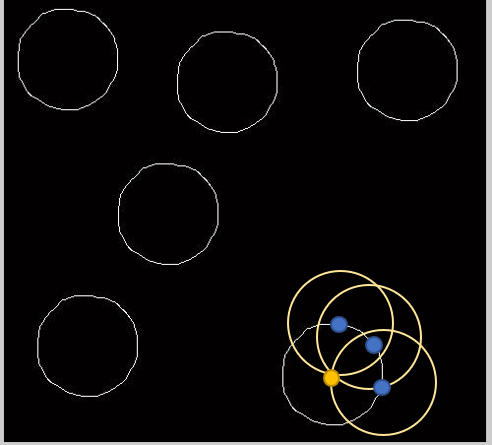
\includegraphics[width=\textwidth]{imgs/q1_81.png}
	\caption{CHT algorithm on pixels}
  \end{subfigure}
	\hfill
  \begin{subfigure}{0.4\linewidth}
	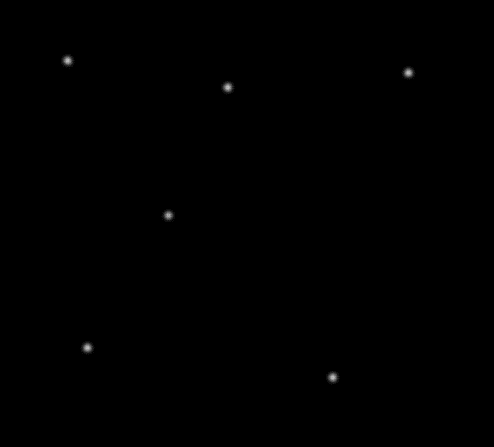
\includegraphics[width=\textwidth]{imgs/q1_82.png}
	\caption{CHT plane}
  \end{subfigure}
\caption{Finding the circles on an image through CHT transform}
\end{figure}
\vskip 0.1in






\newpage
\section{Question 2.}
\subsection{}
The correspondence is the following:
\begin{enumerate}
\item $g_{1} \rightarrow Hf$ - is the following Blur operation. No noise.
\item $g_{2} \rightarrow f + N$ - only Noise is added
\item $g_{3} \rightarrow f$ - is the same as input
\item $g_{4} \rightarrow Hf + N$ - input is blurred, and noise is added.
\end{enumerate}


\subsection{}
Both quality measures $E_b$ and $E_a$ measure the norm of the gradient in an image. First, two major points which help us to solve the question:
\begin{enumerate}
\item Blurring - \textit{decreases} the absolute value of the gradient. Thus, it will decrease both the first and second norm of the gradient.
\item Noise - is a random signal which is added. which increases both the first (TV) and second norm of the gradient. Second norm is increased more, since the gradient value there is squared.
\end{enumerate}

Thus, the result is the following:
\begin{equation*}
\begin{cases}
E_{a}(g_{1}) < E_{a}(g_{3}) \textbf{ ? } E_{a}(g_{4}) < E_{a}(g_{2})  \\
E_{b}(g_{1}) < E_{b}(g_{3}) \textbf{ ? } E_{b}(g_{4}) < E_{b}(g_{2}) 
\end{cases}
\end{equation*}

I have written the '\textbf{?}' mark between images $g_{3}$ and $g_{4}$ in both cases, since we don't have information on the blurring level, and the noise model. Blurring decreases $E_{a}$ and $E_{b}$, but noise increases both of them.







\newpage
\section{Question 5.}
We are looking for a way to maximize each of the priors (those are PDFs).
\newline
The correspondence is the following:
\begin{enumerate}
\item what is measured here is the gradient value in the X direction, multiplied by the pixel value. 
	\begin{itemize}
	\item the most probable priors (which maximizes this expression) are images A,B (has no gradient, all $D_x$ values are 0). 
	\item The most unprobable prior is image F which has a lot of sharp gradients. (where it passes from black to white the pixel value is 1)
	\end{itemize}
\item here both gradients are taken into consideration, and also the pixel value.
	\begin{itemize}
	\item the most probable priors is image C, which has no gradients, and its pixel values are 0. This whole expression will be 0 for it.
	\item The most unprobable prior is image A. Its pixel values are at maximum, and also it has no gradients (which come here with opposite sign, which means that more gradients is good for probability)
	\end{itemize}
\item similarly to case 1, we look here at the gradients in the direction Y.
	\begin{itemize}
	\item Similarly to 1, the most probable images are the ones with no gradients in the Y direction, which are A, C, F
	\item The most unprobable prior is now G (E may have approximately same value), which has gradients on the pixels which have non-zero value, meaning it will decrease the probability.
	\end{itemize}
\item Here we are looking for the biggest pixel values.
	\begin{itemize}
	\item Image A is the most probable, it has the maximum amount of biggest value (white=1) pixels
	\item Image B is the most unprobable.
	\end{itemize}
\end{enumerate}





\includepdf[pages=-]{046200_q3_4.pdf}

\end{document}



















